\documentclass[output=paper,colorlinks,citecolor=brown,
% hidelinks,
% showindex
]{langscibook}

\author{David Alan Hair\affiliation{University of North Georgia} and J. C. Tiegs\affiliation{University of Arizona}\orcid{https://orcid.org/0000-0002-0788-8917}}
\title{\textit{¡Me recontra encanta el Twitter!} A quantitative look at online use of intensifier \textit{recontra} in Argentine and Peruvian Spanish}

\abstract{ This paper presents a quantitative analysis of the use of \textit{recontra} as an intensifier on the social media application, Twitter, in which we compare Argentine and Peruvian varieties of Spanish. In early examples of \textit{recontra} as an intensifier, it fulfills the same syntactic and semantic function as \textit{muy} and could be substituted by other intensifiers in Spanish such as \textit{re} or \textit{súper}. In more recent tokens of \textit{recontra}, its use is not limited to these cases, but extends to pre-verbal collocation where it exercises a unique intensifier function that cannot be substituted with a canonical adverb. We describe the grammaticalization of \textit{recontra} as an intensifier and interpret the syntactic freedom of its use in the two varieties of Spanish. The data suggest varying semantic interpretations of the use of \textit{recontra} as well as statistically significant differences by region based on the polarity of the utterance in which the intensifier appears.}

\IfFileExists{../localcommands.tex}{%hack to check whether this is being compiled as part of a collection or standalone
   % add all extra packages you need to load to this file

\usepackage{tabularx,multicol,multirow}
\usepackage{url}
\urlstyle{same}

\usepackage{listings}
\lstset{basicstyle=\ttfamily,tabsize=2,breaklines=true}

\usepackage{langsci-basic}
\usepackage{langsci-optional}
\usepackage{langsci-lgr}
\usepackage{langsci-gb4e}
%    \let\eachwordone=\it % Ch 14, 18

\usepackage{jambox}
\usepackage{subfigure}
\usepackage{tablefootnote}
\usepackage[nameinlink, noabbrev]{cleveref}
\crefname{enumi}{example}{examples}

\usepackage{bbding}
%\usepackage{linguex}
\usepackage{stmaryrd}

\usepackage{tipa}
\let\ipa\textipa
\usepackage{vowel}
\newcommand{\BlankCell}{}
\usepackage{ot-tableau}

\usepackage{forest}
\useforestlibrary{linguistics}
\usepackage[noeepic]{qtree}
\usepackage{pstricks, pst-xkey, pst-jtree}
\usepackage{tikz-qtree}
\usepackage{tikz-qtree-compat}
\usepackage{tree-dvips}

\usepackage{lastpage}
\usepackage{hyperref}
\usepackage{xltxtra}

\usepackage{ragged2e}
%\usepackage{subcaption}
\usepackage{floatrow}
\usepackage{float}

\usepackage[normalem]{ulem} % Pour les textes barrés
\usepackage{ifthen} 

\usepackage{todonotes}

   \newcommand*{\orcid}{}

\makeatletter
\let\theauthor\@author
\makeatother

\papernote{\scriptsize\normalfont
    \theauthor.
    \titleTemp. 
    To appear in: 
    Chad Howe and Pilar Chamorro and Timothy Gupton and Margaret Renwick.
    Theory, Data, and Practice: Selected papers from the 49th Linguistic Symposium on Romance Language
    Berlin: Language Science Press. [preliminary page numbering]
}

% Workaround for subscripts with capital letters
\newcommand{\capsub}[1]{\ensuremath{_\text{#1}}}

% Chapter 10: Table-like presentation within example environment
% classical latin > {*}late latin > old french  earlier > later   gloss
\newcommand{\montanoboxi}[7]{\parbox{2cm}{#1} > {#2}\parbox{2cm}{#3} > \parbox{1.5cm}{\textit{#4}} \parbox{1.2cm}{#5}\ > \parbox{1.2cm}{#6} \parbox{1.5cm}{#7}}
% {*}latin > earlier OF [ipa] > early OF   gloss
\newcommand{\montanoboxii}[6]{{#1}\parbox{1.9cm}{\textit{#2}} > \parbox{1.3cm}{\textit{#3}} \parbox{2cm}{#4} \parbox{2cm}{#5} \parbox{1.9cm}{#6}}

% Chapter 5
\newcommand{\redc}[1]{\textcolor{red}{#1}}
\newcommand{\bluec}[1]{\textcolor{blue}{#1}}
\newcommand{\ajout}[1]{\textcolor{blue}{#1}}
\newcommand{\ajoutplus}[1]{\textcolor{cyan}{#1}}

\newcommand{\hachure}[9]{
% Parametres :
% Coordonnees bas gauche (2 parametres) : (#1,#2)
% Coordonnees haut droit (2 parametres) : (#3,#4)
% Orientation : #5
%   1 : diagonale de pente 1
%  -1 : diagonale de pente -1
%   0 : horizontal
%   2 : vertical
% Nombre de pas horizontaux : #6
% Epaisseur du trait : #7
% Couleur : #8 (ex. green)
% Atténuation couleur : #9 (ex. 30)
\pgfmathsetmacro{\N}{#6-1}
\pgfmathsetmacro{\A}{#1}
\pgfmathsetmacro{\B}{#2}
\pgfmathsetmacro{\C}{#3}
\pgfmathsetmacro{\D}{#4}
\pgfmathsetmacro{\I}{(#3-#1)/#6}
\pgfmathsetmacro{\J}{(#4-#2)/#6}
\ifthenelse{\equal{#5}{1}}{
  \foreach \n in {0,...,\N}
    \foreach \m in {0,...,\N}
      {
        \pgfmathsetmacro{\X}{\A + ((0 + \n) * \I)}
        \pgfmathsetmacro{\Y}{\B + ((0 + \m) * \J)}
        \pgfmathsetmacro{\U}{\A + ((1 + \n) * \I)}
        \pgfmathsetmacro{\V}{\B + ((1 + \m) * \J)}
        \draw[#8!#9,#7] (\X, \Y)--(\U, \V);
      } 
  }{}
\ifthenelse{\equal{#5}{-1}}{
  \foreach \n in {0,...,\N}
    \foreach \m in {0,...,\N}
      {
        \pgfmathsetmacro{\X}{\A + ((1 + \n) * \I)}
        \pgfmathsetmacro{\Y}{\B + ((0 + \m) * \J)}
        \pgfmathsetmacro{\U}{\A + ((0 + \n) * \I)}
        \pgfmathsetmacro{\V}{\B + ((1 + \m) * \J)}
        \draw[#8!#9,#7] (\X, \Y)--(\U, \V);
      } 
  }{}
\ifthenelse{\equal{#5}{0}}{
  \foreach \n in {0,...,\N}
    \foreach \m in {0,...,\N}
      {
        \pgfmathsetmacro{\X}{\A + ((0 + \n) * \I)}
        \pgfmathsetmacro{\Y}{\B + ((0 + \m) * \J)}
        \pgfmathsetmacro{\U}{\A + ((1 + \n) * \I)}
        \pgfmathsetmacro{\V}{\B + ((0 + \m) * \J)}
        \draw[#8!#9,#7] (\X, \Y)--(\U, \V);
      } 
  }{}
\ifthenelse{\equal{#5}{2}}{
  \foreach \n in {0,...,\N}
    \foreach \m in {0,...,\N}
      {
        \pgfmathsetmacro{\X}{\A + ((0 + \n) * \I)}
        \pgfmathsetmacro{\Y}{\B + ((0 + \m) * \J)}
        \pgfmathsetmacro{\U}{\A + ((0 + \n) * \I)}
        \pgfmathsetmacro{\V}{\B + ((1 + \m) * \J)}
        \draw[#8!#9,#7] (\X, \Y)--(\U, \V);
      } 
  }{}
}

%Définition d'un pattern de type hachure
% \usetikzlibrary{patterns}
% \makeatletter
% \tikzset{hatch distance/.store in=\hatchdistance,hatch distance=5pt,hatch thickness/.store in=\hatchthickness,hatch thickness=5pt}

% \pgfdeclarepatternformonly[\hatchdistance,\hatchthickness]{north east hatch}% name
%     {\pgfqpoint{-\hatchthickness}{-\hatchthickness}}% below left
%     {\pgfqpoint{\hatchdistance+\hatchthickness}{\hatchdistance+\hatchthickness}}% above right
%     {\pgfpoint{\hatchdistance}{\hatchdistance}}%
%     {
%         \pgfsetcolor{\tikz@pattern@color}
%         \pgfsetlinewidth{\hatchthickness}
%         \pgfpathmoveto{\pgfqpoint{-\hatchthickness}{-\hatchthickness}}       
%         \pgfpathlineto{\pgfqpoint{\hatchdistance+\hatchthickness}{\hatchdistance+\hatchthickness}}
%         \pgfusepath{stroke}
%     }
% \pgfdeclarepatternformonly[\hatchdistance,\hatchthickness]{north west hatch}% name
%     {\pgfqpoint{-\hatchthickness}{-\hatchthickness}}% below left
%     {\pgfqpoint{\hatchdistance+\hatchthickness}{\hatchdistance+\hatchthickness}}% above right
%     {\pgfpoint{\hatchdistance}{\hatchdistance}}%
%     {
%         \pgfsetcolor{\tikz@pattern@color}
%         \pgfsetlinewidth{\hatchthickness}
%         \pgfpathmoveto{\pgfqpoint{\hatchdistance+\hatchthickness}{-\hatchthickness}}
%         \pgfpathlineto{\pgfqpoint{-\hatchthickness}{\hatchdistance+\hatchthickness}}
%         \pgfusepath{stroke}
%     }
% \makeatother
%~~~~~~~~~~~~~~~~~~~~~~~~~~~~~~~~~~~~~


% Chapter 7
\newcommand\pef[1]{(\ref{#1})}

\newcommand{\subscript}[1]{\textsubscript}

   %% hyphenation points for line breaks
%% Normally, automatic hyphenation in LaTeX is very good
%% If a word is mis-hyphenated, add it to this file
%%
%% add information to TeX file before \begin{document} with:
%% %% hyphenation points for line breaks
%% Normally, automatic hyphenation in LaTeX is very good
%% If a word is mis-hyphenated, add it to this file
%%
%% add information to TeX file before \begin{document} with:
%% %% hyphenation points for line breaks
%% Normally, automatic hyphenation in LaTeX is very good
%% If a word is mis-hyphenated, add it to this file
%%
%% add information to TeX file before \begin{document} with:
%% \include{localhyphenation}
\hyphenation{
anaph-o-ra
Dor-drecht
%FFI2016-76045-P-AEI/-MINEICO/-FEDE
}

\hyphenation{
anaph-o-ra
Dor-drecht
%FFI2016-76045-P-AEI/-MINEICO/-FEDE
}

\hyphenation{
anaph-o-ra
Dor-drecht
%FFI2016-76045-P-AEI/-MINEICO/-FEDE
}

    \bibliography{localbibliography}
    \togglepaper[23]
}{}

\begin{document}
\maketitle

\section{Introduction}
In the current study, we present a quantitative analysis of digital data from the application Twitter (2018), where we find evidence of innovative linguistic use of the intensifier recontra in two varieties of Latin American Spanish. Written corpora trends (from the Corpus del Español (CdE) and CORPES XXI) indicate that the synchronic use of recontra as an intensifier, which as of this writing is not attested in the \textit{Diccionario de la lengua española} of the Real Academia Española \citep{RAECORDE}, is more statistically prevalent in two varieties of Spanish: those of Argentina and Peru. For that reason, the present analysis limits itself to these two regional varieties of written speech; and as the most tokens were found to come from Buenos Aires and Lima, the countries’ respective capital cities, these are the varieties analyzed here. Previous variationist studies on intensification — defined by \cite[372]{munoz2018estrategias} as the 
``linguistic resources that increase the illocutionary strength of speech acts, emphasize the certainty of a clause [proposition] or the confidence of an assertion'' —  have compared the use of \textit{{muy}} and \textit{bien} (cf. \citealt{KanwitSarrió2017}) for a discussion of regional variation between Argentina and Spain) and highlight the rapid change that occurs in intensifier use within speech varieties (e.g. \citet{Tagliamonte2012}). Given the likelihood of innovation as well as the highly regional variation of intensifiers, our selection of Twitter as a virtual corpus, while somewhat novel, allows us to examine written speech that is more informal in nature and as such, more likely to reflect actual changes in progress in spoken language across varieties. It is also important to mention here that there is diachronic evidence dating to the 15th century \citep{RAECORDE} of \textit{la recontra} used as a noun in opposition to \textit{la contra} as well as later use of \textit{¡re-contra!} as an interjection. Both of these historical uses are relevant in order to explain the evolution and extension of \textit{recontra} as an intensifier; however, an in-depth historical analysis is beyond the scope of this study. 

Regarding the relevant syntactic and semantic restrictions of \textit{recontra} as an intensifier, the first written evidence found in the corpora we consulted for this study occurs in 1968 in a Chilean  text by Francisco Gutiérrez which is found in \ref{ex:hair:fishing} below. Rather than give a translation for \textit{recontra} in our meaning glosses, we have marked the position of the intensifier in this example and all that follow. As can be noted, \textit{recontra} could be translated by a variety of intensifiers in English, depending on its syntactic function as well as the polarity of the context. 

\begin{exe}
\ex\label{ex:hair:fishing}
\gll Nos fue \textbf{recontra} bien en la pesca \ldots\\
us.\textsc{dat} go.\textsc{pst.3sg} \textsc{int} well in the fishing \ldots\\
\glt `Our fishing went \textbf{\textsc{int}} well.' \qquad \citep{RAECORDE}
\end{exe}


In this linguistic environment, it can be seen that \textit{recontra} serves the same intensifier function as \textit{muy} `very' and could also be substituted by other intensifiers such as \textit{súper} `super' in many other varieties of Spanish. Even though we see that \textit{recontra} may be used in environments where other intensifiers could be substituted to accomplish an adjectival intensifier function, current use in Argentine and Peruvian Spanish indicates that \textit{recontra} is also found pre-verbally, where it accomplishes a unique intensifier function not possible by other canonical adverbs (e.g. in order to substitute \textit{mal} 
`badly' for \textit{recontra} in \ref{ex:hair:mesita} or \textit{mucho} `a lot' in other contexts, the intensifier would need to be post verbal): 

\begin{exe}
\ex\label{ex:hair:mesita}
\gll Me  estaba	sacando la ropa y me \textbf{recontra} golpie (sic) el   codo   con  la 	mesita de luz \ldots \\
me.\textsc{refl} be.\textsc{pst.ipfv.1sg} take-off.\textsc{prog} the clothes and me.\textsc {refl} \textsc{int} hit. \textsc{pst.1sg} the elbow with the nightstand \ldots \\
\glt `I was taking off my clothes and I \textbf{\textsc{int}} banged my elbow on the nightstand \ldots' \qquad \citep{Twitter:Whatareyoudoing2018}
\end{exe}


In this variationist study, we explore this novel intensifier use in Spanish as conditioned by the linguistic factors of utterance polarity and grammatical class through Twitter data from both speech regions. While geo-tagging in Twitter does not guarantee the originator's geographical speech variety — given that it is impossible to know the linguistic history of each Twitter user regardless of where they may be at the moment of their tweets — we suggest that the aggregate of data does point to regional trends that can be further expanded upon in future corpus analyses of these two geographical regions. Our research questions are as follows: 

\begin{enumerate}
    \item To what extent do the Twitter data reflect the geographical frequency of \textit{recontra} found in other written corpora, namely the \textit{Corpus del español}, CREA and CORPES XXI? 
    \item With which grammatical classes (adjectives/adverbs, nouns, verbs) does \textit{recontra} collocate most in each regional variety (Argentine or Peruvian Spanish)? 
    \item Is there a statistical significance with the use of \textit{recontra} and the polarity of the utterance in which it is found? If so, will this vary according to region or grammatical class? 
\end{enumerate}


Twitter was specifically chosen as the corpus for analysis here due to its casual register and approximation to spoken language use as well as the lack of entries in traditional corpora of \textit{recontra} as an intensifier. Before presenting our methodology and results, the following section summarizes the relevant literature and background regarding the use of \textit{recontra} in Spanish which led us to formulate our research questions regarding the behavior of this novel intensifier. 

\section{Background}\label{sec:hair:2}

Among the few mentions of \textit{recontra} in the previous literature, we begin with an explanation of \ref{ex:hair:whore} and its abbreviated version \ref{ex:hair:birth} below, which point to a diachronic collocation of \textit{recontra} with a common Rioplatense Spanish insult: 


\begin{exe}
\ex\label{ex:hair:whore}
\gll ¡La \textbf{re}putísima madre que te \textbf{recontra} \textbf{mil} parió! \\
the \textsc{int}.whore mother that you.\textsc{acc} \textsc{int} \textsc{int} birth.\textsc{pst.3sg}\\
\glt `Your \textbf{\textsc{int}} whore of a mother that \textsc{int} \textsc{int} birthed you!' \citep[78]{Teruggi1981}
\end{exe}

\begin{exe}
\ex\label{ex:hair:birth}
\gll ¡Que te \textbf{recontra}! \\
that you.\textsc{acc} \textsc{int}\\
\glt `That \textbf{\textsc{int}} (birthed) you!' \citep[78]{Teruggi1981}\\
\end{exe}

Teruggi explains the subtleties of this insult and assures us that they spring from the Argentine variety of Spanish. If this is indeed the case, it is not surprising that \textit{recontra} is found to collocate pre-verbally in this variety of Spanish; however, no data are given to support these claims. Even so, other authors also attribute the origins of \textit{recontra} to the Rioplatense or Southern Cone regions of South America more generally \citep{Rabanales1958,kornfeld2012cuantificacion,resnik2012gramaticalizacion}. As this paper does not attempt a diachronic explanation of \textit{recontra}, we will refrain from speculating on its exact origin, while still analysing its synchronic use according to the data available to us. As we saw in \ref{ex:hair:fishing} above, the first written evidence found of \textit{recontra} as an intensifier comes from a Chilean manuscript from 1968. \citet{martin1998prefijos} quotes \citet{Rabanales1958} in attributing the intensifier use of \textit{recontra} to a Chilean phenomenon denoting a greater degree of intensity to the prefix \textit{re} \citep[113]{martin1998prefijos}. \citet[73]{kornfeld2012cuantificacion} maintains that \textit{recontra} is an Argentine and Uruguayan phenomenon and is a variant along with \textit{requete} of the very common intensifier \textit{re} as well. At the current writing, there are very few mentions (c.f. Cerrón-Palomino 2015; Castro Lizares 2016) in the literature that associate the use of \textit{recontra} specifically with the Peruvian variety of Spanish and we suggest that a diachronic study is vital to determine the origins of \textit{recontra} in this region and whether they are due to contact or if they might represent a form of parallel lexical evolution. 

\citet{kornfeld2012cuantificacion} compares \textit{re} in the Rioplatense region with \textit{ité} in Paraguayan Spanish (in contact with Guaraní) from a generativist perspective. Among the casual mentions of \textit{recontra} in her work, she suggests that its use is restricted to an oral register, which would help explain its higher prevalence in the Twitter data as compared to CORPES XXI data. However, the fact that \textit{recontra} is found in these written media (albeit informal registers) questions her assertion that it is limited to the oral register alone and could indicate that there is a change in progress in which \textit{recontra} is becoming more accepted in written as well as spoken language.  

Another aspect of \citeauthor{kornfeld2012cuantificacion}'s study is her analysis of the use of \textit{re} with telic verbs (denoting achievement/accomplishment). She finds that \textit{re} can be used in these cases where it indicates the idea of completeness (e.g. can be substituted by \textit{completamente} `completely') \citep[73--75]{kornfeld2012cuantificacion}. On the other hand, she proposes that \textit{recontra}, in opposition to \textit{re}, is less flexible syntactically and that it is only permitted to collocate with verbs when its meaning could be substituted by \textit{mucho} `a lot’. However, all of her examples are with \textit{re} and not \textit{recontra}, therefore one of the goals of the current study is to discover qualitative data about the syntactic restrictions of \textit{recontra} in order cultivate further areas of analysis.

\citet[103]{martin1998prefijos}, in her study of prefix intensifiers, among them \textit{re, archi, mega}, etc., discusses the idea of polarity and maintains that this depends on the semantic content of the utterance in which the intensifier is found, not on any intrinsic properties of the intensifiers themselves. This idea of the intensifier as being semantically free from polarity constraints is an interesting point of departure in analyzing \textit{recontra}, since one of its uses (see Teruggi 1981) is notably negative in that it springs from a rather vitriolic insult about one’s mother. In this light, examining the polarity of \textit{recontra} will help in determining its evolution and extension toward a canonical (semantically at least) status as an intensifier. Similar to what we have seen with \citeauthor{kornfeld2012cuantificacion}’s analysis above (with the exception of \textit{re}), \citeauthor{martin1998prefijos} also asserts that only atelic verbs may be intensified, allowing intensification of each stage of an action, rather than telic verbs that indicate finality, giving us further reason to test the syntactic flexibility of \textit{recontra} in the data of the current study. 

In the present study a distinction must be drawn between free and bound morphemes. In its use with verbs, \textit{re} clearly functions as a bound morpheme as affixes are by definition bound to the verb they are modifying \citep{EscobarHualde}. However, while \textit{recontra} can be bound to a modified verb as in \ref{ex:hair:crossfit}, it is also found in isolation, unbound to other morphemes \ref{ex:hair:enamoradiza}. This behavior suggests that \textit{recontra} can function as a free morpheme, allowing it liberties not enjoyed by affixes like \textit{re} whose historical origins are also prefixal in nature. This distinction is important in that it may play a role in its potential syntactic freedom. 

\begin{exe}
\ex\label{ex:hair:crossfit}
\gll Me \textbf{recontra} duelen los bíceps de Crossfit \ldots \\
\textsc{dat.1sg} \textsc{int} hurt.\textsc{prs.3pl} the biceps from Crossfit \ldots \\
\glt `My biceps \textbf{\textsc{int}} hurt from Crossfit \ldots' \citep{Twitter:Whatareyoudoing2018}\\
\end{exe}

\begin{exe}
\ex\label{ex:hair:enamoradiza}
\gll ¿Sos muy enamoradiza? \\
be.\textsc{prs.2sg} very prone-to-fall-in-love \\
\gll -- \textbf{Recontra}. Pero ahora soy más exigente. \\
-- \textsc{int}    but now be.\textsc{prs.1sg} more picky \\
\glt `Do you fall in love easily? -- \textbf{\textsc{int}}. But now I'm pickier.' \citep{Davies2016}\\
\end{exe}

While \textit{re} can be bound by its historical use with verbs to imply iteration, \textit{recontra} does not seem to have this reading. In addition, \textit{recontra} is composed of two morphemes (\textit{re} and \textit{contra}), further distinguishing it from single morphemic \textit{re} as well as \textit{súper}. 

This unique status may be important in its relatively rapid extension and evolution in the varieties of Spanish where it is used as an innovative intensifier with ambiguous semantic associations (telic/atelic, repetitive/quantifiable, etc.). This semantic-pragmatic extension is an early step in the process of grammaticalization \citep{HopperTraugott2003,HeineNarrog2010}. Grammaticalization -- the change of a lexical item to a (more) grammatical or functional element \citep{HopperTraugott2003} -- is often thought to follow a path that includes pragmatic extension followed by 
`semantic bleaching' \citep{TraugottBerndHeine1991,CampbellJanda2001,HeineNarrog2010}), which involves a loss or generalization of meaning. We will explore grammaticalization as it relates to the extension of \textit{recontra} as an intensifier in the discussion section. 

Regarding the research questions from our introduction, the previous literature does not provide much direction for developing clear hypotheses since there is little mention of \textit{recontra} in general. A comparison with the other intensifiers analyzed in the literature is also difficult to approach given the morphological differences (prefix vs. free morpheme) between prefixal intensifiers like \textit{re} or \textit{súper} and \textit{recontra}. In addition, there is a lack of data regarding the possibilities for intensifier collocation based on its modifying a particular grammatical class (adjectival/adverbial, substantival, verbal), except for a brief mention by \citet{kornfeld2012cuantificacion} that \textit{recontra} may only be used when it can be interpreted to mean \textit{mucho} 'a lot'. Regarding polarity, since there is no clear indication that intensifiers are preferred in either positive or negative contexts, our hypothesis is that there should be no significant difference based on polarity, either in association with region or grammatical class. However, given the possibility that one of the original uses of \textit{recontra} in Rioplatense Spanish was in combination with an insult, it is possible that the data will indicate a preference for negative polarity in its use, at least in the Argentine variety of Spanish.

\section{Methodology}

Besides our initial cursory diachronic search of \textit{recontra} mentioned above, we began our analysis with a synchronic investigation regarding the use of \textit{recontra} in three distinct written corpora before continuing with the Twitter data portion of this study. In \tabref{tab:hair:1:frequencies}, the frequencies are given for the use of \textit{recontra} in both Argentina and Peru, out of total tokens of \textit{recontra}, according to the 3 written corpora used. As can be seen from the total tokens listed in \tabref{tab:hair:1:frequencies}, the \textit{Corpus del Español} \citep{Davies2016} contained by far the most written evidence of the use of \textit{recontra}, which can be explained by the size of this online corpus, which contains 2 billion total words from around 2 million web pages from 21 Spanish-speaking countries. After Argentina and Peru, the next 3 countries where the most uses of \textit{recontra} were found were Uruguay (n=258), Mexico (n=135) and Spain (n=113). While an analysis of more regions is needed to increase our understanding of the variable use of \textit{recontra} in all varieties of Spanish, we have limited the current analysis to Argentina and Peru for the sake of brevity and as our point of departure for future work in this area of inquiry. In each corpus, we find that overall frequency is categorically higher in Peru in comparison with Argentina. Even though this is an overall frequency based solely on three written corpora, we should highlight here that since more mentions of \textit{recontra} in the previous literature are associated with Argentine or Rioplatense Spanish than Peruvian Spanish, the fact that it appears more frequently in Peruvian Spanish in these data is of great interest and may indicate a change in progress in this variety. 


\begin{table}
\caption{Frequency comparison of \textit{recontra} in Argentina and Peru}
\label{tab:hair:1:frequencies}
 \begin{tabular}{l rr}
  \lsptoprule
             & Argentina & Peru\\
  \midrule
  Corpus del Español \citep{Davies2016} & 20\% (N=605) & 46\% (N=1390)\\
  CREA \citep{RAECREA}  & 21\% (N=4) & 42\% (N=8)\\
  CORPES XXI \citep{RAECORDE} & 23\% (N=12) & 34\% (N=18)\\
  \lspbottomrule
  \end{tabular}
\end{table}

While these corpora provided a base understanding of frequency of \textit{recontra} use from web-pages originating in these countries, our quantitative analysis focuses on Twitter data, which are geo-tagged for location of users. \tabref{tab:hair:2:tokens} gives the overall tokens of \textit{recontra} in Argentina and Peru during a consecutive 7-day period of Twitter data mining. Here, in contrast to what we have seen with the other three written corpora, it is in Argentina where more tokens are found of this intensifier. As we mentioned in the introduction, the geo-tagging used in order to classify the Twitter data does not definitively show that the language user is from the particular region tested, although the same could be said for many publicly available written corpora as well, such as the \textit{Corpus del Español}, for which specific user background data are also unavailable. 

\begin{table}
\caption{Tokens of \textit{recontra} by country from Twitter: 9-april-2018 to 15-april-2018}
\label{tab:hair:2:tokens}
 \begin{tabular}{l r}
  \lsptoprule
             & \% of Total tokens \\
  \midrule
  Argentina & 71\% (n=1157)\\
  Peru  & 29\% (n=470)\\
  Total & n=1627\\
  \lspbottomrule
  \end{tabular}
\end{table}

In order to find and extract these Twitter data, the package twitteR for RStudio was used in combination with the first author's Twitter Developer application. During this process, RStudio was used to search for tweets within a radius of 100 kilometers of each country's capital: Buenos Aires (Argentina) and Lima (Peru). The data were extracted automatically, tabulated and then coded by the first author before being verified by the second author. The present study considers the first 100 tokens from each country's data extraction. Extracted data where \textit{recontra} appeared in the user name field or where the same token had been retweeted were excluded before selecting the first 100 tokens. Apart from this procedure, no other data were excluded. 
 
 In evaluating the 200 tweets used as the corpus for this study, we first coded them according to collocation with an adjective/adverb (A), a noun (S) or a verb (V). In regard to polarity, each tweet was assigned either a tag of positive (P), negative (N) or neutral (0), according to the semantic reading of the elements modified by the intensifier \textit{recontra}. The criterion used to determine positive and negative polarity was a test of whether the related utterance would indicate that \textit{a person should be praised for action or description X or not}, adapted from Wachter's tests regarding the felicity of the 
``pragmatic behavior of adjectives'' \citep[12]{Wachter2012}. If that question could not be answered affirmatively or negatively, a neutral designation was assigned. In the case of obscene speech or insults, negative polarity was assigned. In \ref{ex:hair:feliz} below, we highlight examples of sample  types of utterances from the Twitter data according to grammatical class and polarity. 


\begin{exe}
\ex\label{ex:hair:feliz}
\begin{xlist}
\ex 
Adjective/Adverb-positive:\\
\gll ¿Estás \textbf{recontra} feliz porque Perú va al mundial?\\ 
be.\textsc{prs.2sg} \textsc{int} happy because Peru go.\textsc{prs.3sg} to-the global\\
\glt `Are you \textbf{\textsc{int}} happy because Peru is going to the World Cup?' (Peru)\\
\ex
Noun-negative:\\
\gll \ldots Ese si(sic) era un \textbf{recontra} \#pajero\\
that.\textsc{subj.dem} yes be.\textsc{pst.ipfv.3sg} a \textsc{int} jerk-off\\
\glt `That guy really was a \textbf{\textsc{int}} jerk-off' (Peru)\\ 
\end{xlist}
\end{exe}


\section{Results}

In Figures 1 and 2 below, the Twitter data results are shown by country and collocation of \textit{recontra} by grammatical class. Upon initial inspection, a much greater use of \textit{recontra} can be seen in the Peruvian variety of Spanish in combination with adjectives/adverbs as compared to other grammatical classes. In the Argentine variety, there is nearly equal collocation with verbs as compared to adjectives/adverbs and in both varieties, there is much less collocation with nouns. In \figref{fig:hair:3}, these results are compared and a chi-square test indicates a statistical significance by grammatical class according to country (chi-square: 18.28, p < 0.001), demonstrating that the linguistic factor of grammatical class is relevant in determining the probability of variation in intensifier use by country according to collocation with grammatical class. 

\newpage

\begin{figure}
    
    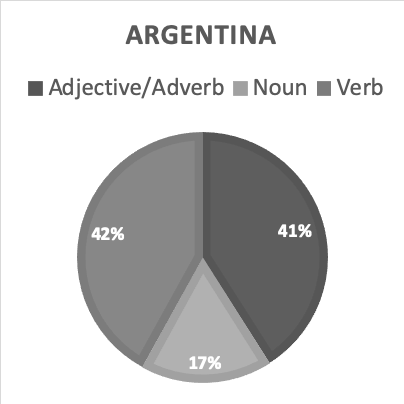
\includegraphics[scale=0.55]{figures/hair_figure1_arg.png}
    \caption{Collocation of 100 tokens of recontra by grammatical class in Argentina}
    \label{fig:hair:1}
\end{figure}

\begin{figure}
    
    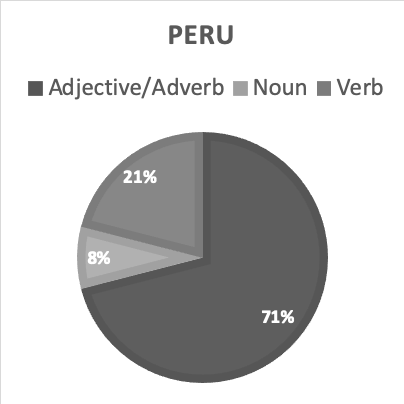
\includegraphics[scale=0.55]{figures/hair_figure2_peru.png}
    \caption{Collocation of 100 tokens of recontra by grammatical class in Peru}
    \label{fig:hair:2}
\end{figure}

\begin{figure}
    
    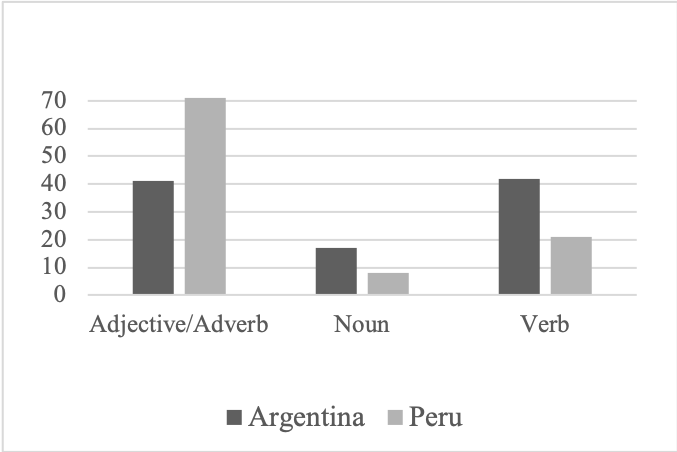
\includegraphics[scale=0.55]{figures/hair_figure3_overall.png}
    \caption{Comparison of overall tokens by country and grammatical class (chi-square: 18.2757. p-value: .00010cross8. Result significant at p < .05)}
    \label{fig:hair:3}
\end{figure}

\newpage


Although this study did not code for further classification of verb types (related to discussion in \citealt{kornfeld2012cuantificacion} mentioned previously regarding telicity), we did note impressionistically a tendency in the Argentine data for \textit{recontra} to be employed more with verbs where it is not possible to get the semantic reading of \textit{mucho} `a lot.' For example, in \ref{ex:hair:payaso} below, we note that \textit{recontra} does not have the interpretation of \textit{mucho} 'a lot,' but rather a more punctual meaning (also confirmed impressionistically by multiple native speakers of Argentine Spanish). This contradicts the conditions that \citet{kornfeld2012cuantificacion} claims constrain its use in comparison to the intensifier \textit{re}.

\begin{exe}
\ex\label{ex:hair:payaso}
\gll @realDonaldTrump Payaso tremendo \ldots Vladimir Putin te va(sic) \textbf{recontra} coger de parado\\
[username] clown tremendous \ldots Vladimir Putin you.\textsc{acc} go.\textsc{prs.3sg} \textsc{int} fuck of standing\\
\glt `@realDonaldTrump you huge clown \ldots Vladimir Putin is going to \textbf{\textsc{int}} fuck you standing up' \citep{Twitter:Whatareyoudoing2018}
\end{exe}

 Regarding the polarity of the environment in which \textit{recontra} occurs, there is no significant difference in use between the two regions as shown by a chi-square test (chi-square: 0.5821, p = 0.75) (see \figref{fig:hair:4} below), although the Peruvian data do indicate a slight advantage for positive collocation in comparison with the Argentine variety. Both regions show equal preference for negative collocation and this is slightly higher than positive use, although  not statistically significant. However, in Figures 5-6 (below), we did find overall differences in polarity based on collocation by grammatical class between the two speech varieties, notably that the two varieties differ in that Argentine verb use collocates more with \textit{positive} utterances and Peruvian use with \textit{negative} utterances. 
 
 
 \begin{figure}
     
     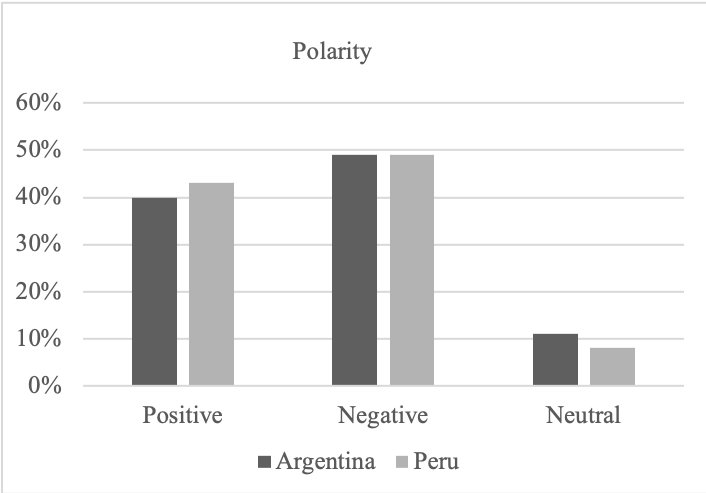
\includegraphics[scale=0.75]{figures/hair_figure4_polarity.png}
     \caption{Polarity of utterance with \textit{recontra} according to variety (chi-square: 0.5821. p-value: .747472. Result not significant at p < .05)}
     \label{fig:hair:4}
 \end{figure}
 
 
 \begin{figure}
     
     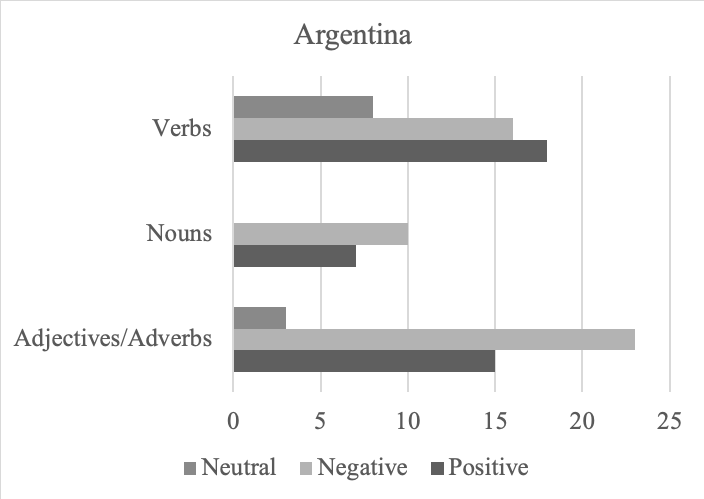
\includegraphics[scale=0.75]{figures/hair_figure5_pol_arg.png}
     \caption{Polarity by grammatical class in Argentina out of 100 tokens of \textit{recontra}}
     \label{fig:hair:5}
 \end{figure}


 \begin{figure}
     
     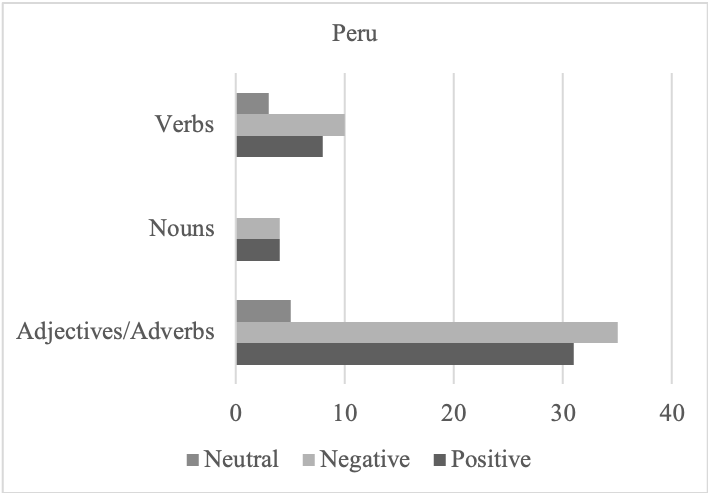
\includegraphics[scale=0.75]{figures/hair_figure6_pol_peru.png}
     \caption{Polarity by grammatical class in Peru out of 100 tokens of \textit{recontra}}
     \label{fig:hair:6}
 \end{figure}
 


Since polarity was not a significant factor overall between the two varieties, it remained to be seen whether the differences based on grammatical class were significant. Chi-square tests were completed to test the significance of collocation by grammatical class according to polarity for each variety of Spanish. In Figures 7-8 below (divided by region and positive/negative polarity) there is a significant difference in relation to grammatical class (chi-square for positive polarity: 10.13, p < 0.05; chi-square for negative polarity: 6.44, p < 0.05). For this portion of the analysis, the neutral utterances were excluded since there were cases where no neutral tokens were found.

\begin{figure}
    
    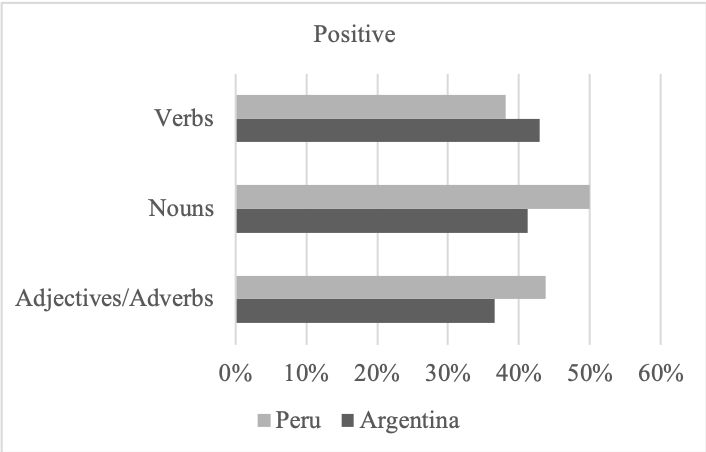
\includegraphics[scale=0.75]{figures/hair_figure7_positive.png}
    \caption{Comparison of frequency of positive collocation according to grammatical class between Argentine and Peruvian Spanish (chi-square: 10.13144. p-value: .0063. Result significant at p < .05)}
    \label{fig:hair:7}
\end{figure}


\begin{figure}
    
    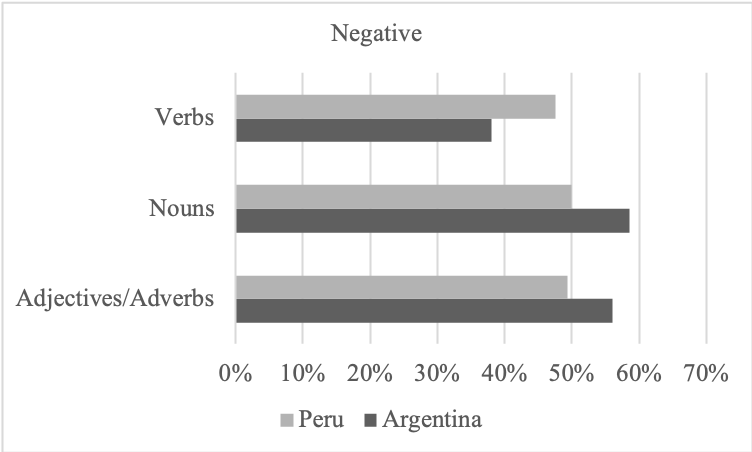
\includegraphics[scale=0.75]{figures/hair_Figure8_negative.png}
    \caption{Comparison of frequency of negative collocation according to grammatical class between Argentine and Peruvian Spanish (chi-square: 6.4388. p-value: .039979. Result significant at p < .05)}
    \label{fig:hair:8}
\end{figure}



\section{Discussion}

In order to draw conclusions based on these data, we repeat our research questions here:

\begin{enumerate}
    \item To what extent do the Twitter data reflect the geographical frequency of \textit{recontra} found in other written corpora, namely the Corpus del Español, CREA and CORPES XXI?  
    \item With which grammatical classes (adjectives/adverbs, nouns, verbs) does \textit{recontra} collocate most in each regional variety (Argentine or Peruvian Spanish)? 
    \item Is there a statistical significance with the use of \textit{recontra} and the polarity of the utterance in which it is found? If so, will this vary according to region or grammatical class?
\end{enumerate}


Regarding the first research question, the Twitter data from the present study diverge from the other corpora that indicate a higher frequency of \textit{recontra} in written Peruvian Spanish in comparison with Argentine Spanish. The fact that our data point to a higher frequency of \textit{recontra} in Argentine Spanish does suggest a higher use of \textit{recontra} in this variety, although not necessarily in all speech registers or communities, given the fact that Twitter is a highly informal written register and our data are limited to a one-week time-frame and geo-tagged only for Buenos Aires and the surrounding area. The results of this study do indicate that regional differences are an important factor in the consideration of the lexical intensifier \textit{recontra} and provide a basis for further questions related to socio-geographical variation. 

In regard to the second research question, we found that grammatical class is a statistically significant factor in describing linguistic behavior related to the use of \textit{recontra} and that this variation can be differentiated at the dialectal level. The main difference noted was a higher collocation with verbs in Argentina in comparison with a higher use with adjectives/adverbs in Peru (see \figref{fig:hair:3} above). In relation to the polarity of the utterance in which \textit{recontra} is found, dialectal variation was also important, although this factor depended on grammatical class to reach statistical significance. In Peru, where in general there were fewer uses of \textit{recontra} with verbs, these tended to be more negative than in Argentina, where collocation with verbs was more frequent and also tended to be used in more positive polarity contexts. From a qualitative standpoint, the examples of verbal collocation in Peru tended to be in combination with obscene speech, which could aid in explaining the evolution of \textit{recontra} in the Peruvian variety and point to a possible further grammaticalization that has taken place in Argentine Spanish, causing \textit{recontra} to be more flexible in a pre-verbal position as well as semantically more distanced from its possible origins as an insult (recall \ref{ex:hair:whore} and \ref{ex:hair:birth} from \sectref{sec:hair:2}). 

The fact that in the data from Peruvian Spanish \textit{recontra} tends to collocate with verbs in negative polarity environments may point to a remnant of its use as an insult in Rioplatense Spanish, suggesting less semantic bleaching than is evident in the Argentine variety. However, diachronic data are needed in order to determine the origins of \textit{recontra} generally and how its use developed in each region. The extent of bleaching that has occurred in the Argentine variety now allows the intensifier to be collocated with verbs more frequently with positive polarity utterances at a higher rate than the Peruvian variety seems to allow. The fact that the majority of tokens of \textit{recontra} from Peruvian Spanish were collocated with adjectives/adverbs, while the Argentine data reflected almost equal tokens collocated with adjectives/adverbs as with verbs (compare Figures 1 and 2), is also an indication that \textit{recontra} is more grammaticalized in the particular variety of Argentine Spanish represented by the data of this study. 

\section{Further directions}

At this point in our research, we find that more work regarding the diachronic development of intensification in both of these varieties of Spanish (and others) that considers processes of grammaticalization, semantic change as well as other linguistic, social or discourse factors, will serve to shed more light on the novelty and extension of \textit{recontra} as an intensifier in both varieties as well as to predict paths for future language variation and change. While our results point to definite processes of grammaticalization and semantic bleaching that allow more syntactic licensing for intensifiers (specifically free morphemes like \textit{recontra}), it seems that the limits of these processes are linked not only to the linguistic factors discussed in this paper, but also to pragmatic constraints that tend to be highly variable according to speech variety. Future studies relating to \textit{recontra} that compare data from spoken (or other written) corpora obtained through controlled, comparable methodologies will allow for conclusions that further explain the synchronic use of this intensifier as well as predict more generalizable trends related to intensification and processes of grammaticalization in general.
 
 

 
 
 
\printbibliography[heading=subbibliography,notkeyword=this]

\end{document}







